\documentclass{beamer}

\usetheme{Copenhagen}
\usecolortheme{beaver}

\usepackage[utf8]{inputenc}
\usepackage{color}
\usepackage{graphics}
\usepackage{graphicx}
\usepackage{wrapfig}
\usepackage{amsmath}
\usepackage{hyperref}
\usepackage{epstopdf}
\bibliographystyle{plain}


\title{Network Computing courses}
\author{Maël Auzias}
\institute{ENSIBS - UBS}
\date{October 2014}

\AtBeginSection[]  % The commands within the following {} will be executed at the start of each section.
{
\begin{frame} % Within each "frame" there will be one or more "slides."  
\frametitle{Presentation Outline} % This is the title of the outline.
\tableofcontents[currentsection]  % This will display the table of contents and highlight the current section.
\end{frame}
} % Do not include the preceding set of commands if you prefer not to have a recurring outline displayed during your$

\begin{document}

\begin{frame}
  \titlepage
  \begin{figure}[p]
      \centering
      
\includegraphics[height=1cm]{./imgs/cc40.jpg}
      \caption{\color{blue}\href{http://teaching.auzias.net}{teaching.auzias.net}}
    \label{fig:cc40}
  \end{figure}
\end{frame}

%\begin{frame}
%\tableofcontents
%\end{frame}

  \begin{frame}
    \frametitle{Course details}
    \begin{columns}
      \column{.5\textwidth}
        \begin{block}{Objectives}
          \begin{itemize}
            \item How do \emph{computers} communicate?
            \item What are the mechanisms \textbf{under} an HTTP request or a telegram message?
            \item Networks are all around us, better study them!
          \end{itemize}
        \end{block}
      \column{.5\textwidth}
        \begin{figure}[t]
          \centering
          
\includegraphics[height=3cm]{./imgs/ntwks.pdf}
          \label{fig:ntwks}
        \end{figure}
    \end{columns}
  \end{frame}

  \begin{frame}
    \frametitle{Course details}
    \begin{columns}
      \column{.3\textwidth}
        \begin{figure}[t]
          \centering
          
\includegraphics[height=4cm]{./imgs/grade.pdf}
          \label{fig:marks}
        \end{figure}
      \column{.7\textwidth}
        \begin{block}{Evaluation}
          \begin{itemize}
            \item Short test at the beginning of every lesson (5 min) ?
            \item Project
            \item Final exam (1 hour)
            \item All same weighting
          \end{itemize}
        \end{block}
        \begin{block}{Material}
          \begin{itemize}
            \item Slides available at \color{blue}\href{http://teaching.auzias.net}{teaching.auzias.net} \color{black} (github too)
          \end{itemize}
        \end{block}
    \end{columns}
  \end{frame}


\section{Introduction}
\subsection{Definitions and presentation}
  \begin{frame}
    \frametitle{Definitions}
      \begin{itemize}
        \item \textbf{Network:} an \textbf{interconnected} group or system\pause
        \item \textbf{Internet:} world wide \textbf{interconnected system of network\emph{s}} \color{blue}\href{http://tools.ietf.org/html/rfc791}{RFC791 (September 1981)}\color{black}\pause
        \item \textbf{IP:} Internet \textbf{Protocol} provides the functions necessary to deliver a package of bits from a source to a destination over a network\pause
        \item \textbf{(world wide) Web:} \textbf{network} consisting of a collection of Internet websites using HTTP
      \end{itemize}
  \end{frame}
  \begin{frame}
    \frametitle{Definitions}
      \begin{itemize}
        \item \textbf{HTTP:} Hypertext Transfer \textbf{Protocol}, application-level protocol for distributed, collaborative, hypermedia information systems \color{blue}\href{http://tools.ietf.org/html/draft-ietf-httpbis-http2-14}{draft HTTP2 (July 2014)} \color{black}\pause
        \item \textbf{FTP:} File Transfer \textbf{Protocol} promotes sharing of files, encourages the use of remote computers \color{blue}\href{http://tools.ietf.org/html/rfc959}{RFC959 (October 1985)} \color{black} \pause
        \item \textbf{TCP:} Transmission Control \textbf{Protocol} is intended for use as a highly reliable host-to-host \color{blue}\href{http://tools.ietf.org/html/rfc761}{RFC761 (January 1980)} \color{black} \pause
        \item \textbf{UDP:} User Datagram \textbf{Protocol} provides  a procedure  for application  programs  to send messages  to other programs  with a minimum  of protocol mechanism \color{blue}\href{http://tools.ietf.org/html/rfc768}{RFC768 (August 1980)} \color{black} \pause
        \item \textbf{RFC:} Request For Comments (Internet Draft (ID), RFC, Internet Standard)
      \end{itemize}
  \end{frame}
  \begin{frame}
    \frametitle{Definitions}
      \begin{itemize}
        \item \textbf{Router:} network \textbf{hardware} providing routing services\pause
        \item \textbf{Routing:} \textbf{algorithm processed} to decide where to forward a packet\pause
        \item \textbf{Forwarding:} \textbf{\emph{action}} of moving a packet from one NIC to another\pause
        \item \textbf{NIC:} Network Interface Card
        \item \textbf{Switch (hub):} network \textbf{hardware} connecting systems using packet switching\pause
        \item \textbf{Packet switching:} forward-like method regardless of the content (destination-based)\pause
        \item \textbf{NAT:} Network Address Translation, router modifying IP address into another IP address.
      \end{itemize}
  \end{frame}
  \begin{frame}
    \frametitle{Definitions}
      \begin{itemize}
        \item \textbf{Node (network):} any entity that can send packets to/receive packets from a network through a NIC\pause
        \item \textbf{Client:} \textbf{computer} able to send requests to a server\pause
        \item \textbf{Request:} \textbf{application message} destined for a server (\emph{order})\pause
        \item \textbf{Server:} \textbf{computer} able to respond a client's requests\pause
        \item \textbf{Request:} \textbf{application message} destined for a client (\emph{result})\pause
        \item \textbf{Fat client:} \textbf{application} where most functions are processed by the client itself\pause
        \item \textbf{Thin client:} \textbf{application} where most functions are carried out on a central server
      \end{itemize}
  \end{frame}

\subsection{Network classification}
  \begin{frame}
    \frametitle{What kind of network is it?}
      \begin{itemize}
        \item \textbf{BAN:} Body Area Network\pause
        \item \textbf{PAN:} Personal Area Networks\pause
        \item \textbf{(W)LAN:} (Wireless) Local Area Networks (home, office, school or airport)\pause
        \item \textbf{MAN:} Metropolitan Area Networks, can cover a whole city\pause
        \item \textbf{WAN:} Wide Area Networks cover a broad area (Internet)
      \end{itemize}
  \end{frame}
  \begin{frame}
    \frametitle{Topologies}
    \begin{figure}[t]
      \centering
      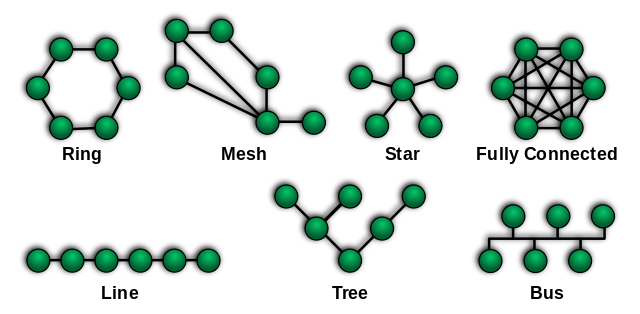
\includegraphics[height=5cm]{./imgs/topologies.png}
      \caption{\color{blue}\href{https://upload.wikimedia.org/wikipedia/commons/thumb/9/97/NetworkTopologies.svg/640px-NetworkTopologies.svg.png}{upload.wikimedia.org}}
      \label{fig:ntwks}
    \end{figure}
      \end{frame}
  \begin{frame}
    \frametitle{Topologies}
    \begin{itemize}
      \item \textbf{Point-to-point:} two entities directly connected to each other (tunnel).\pause
      \item \textbf{Ring:} data go around the ring, unidirectional way network.\pause
      \item \textbf{Mesh:} all nodes cooperate in the distribution of data in the network\footnote{\color{blue}\href{http://www.newscientist.com/article/dn26285-hong-kong-protesters-use-a-mesh-network-to-organise.html}{Hong Kong protesters use a mesh network to organize}}.\pause
      \item \textbf{Star:} all messages go through the same central node, reducing network failure.\pause
      \item \textbf{Fully connected:} all nodes are connected to all other nodes.\pause
      \item \textbf{Line:} bidirectional link between two nodes. Node can only send packet going through its neighbors.\pause
      \item \textbf{Bus:} all nodes are connected to the same media. Only one can send a packet at a time, which all others then receive.\pause
      \item \textbf{Tree:} hierarchical topology, such as a binary tree.
    \end{itemize}
  \end{frame}
  \begin{frame}
    \frametitle{Bonus}
    \begin{figure}[p]
      \centering
      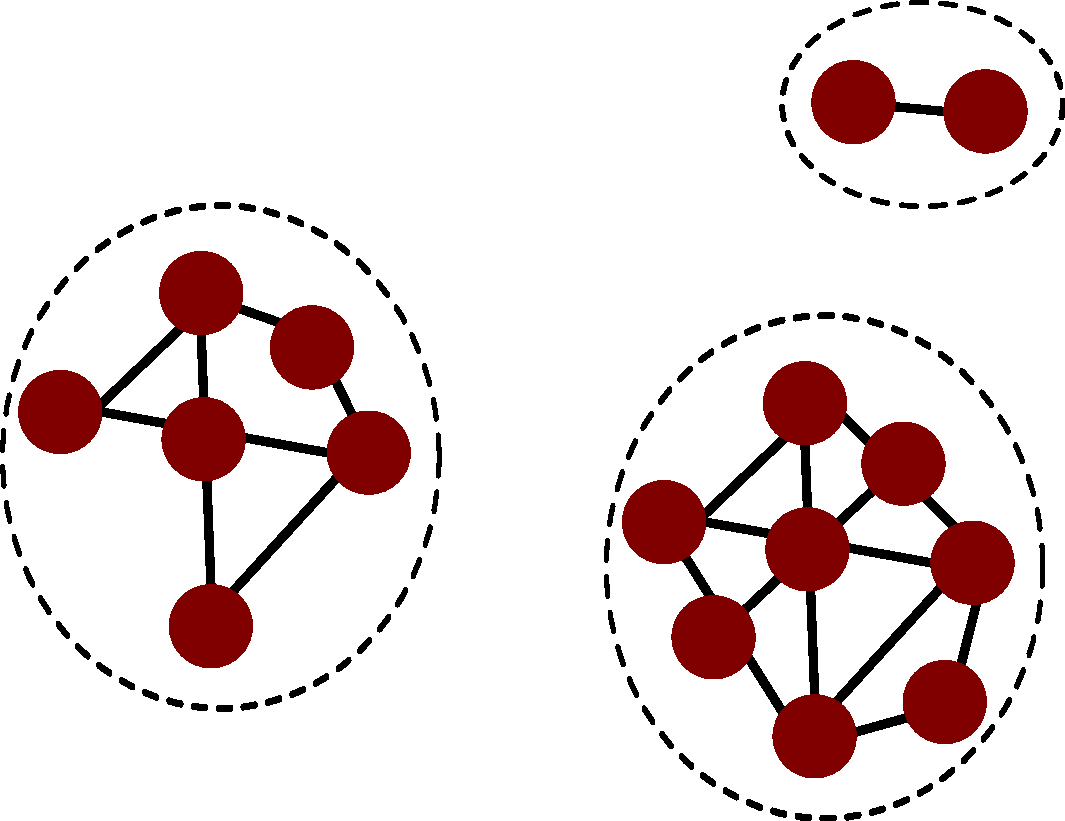
\includegraphics[height=3cm]{./imgs/dmanet.pdf}
      \caption{Disconnected MANET illustration \cite{ieee12khabbaz}}
      \label{fig:dmanet}
    \end{figure}
  \end{frame}
  \begin{frame}
    \frametitle{Bonus}
    \begin{figure}[p]
      \centering
      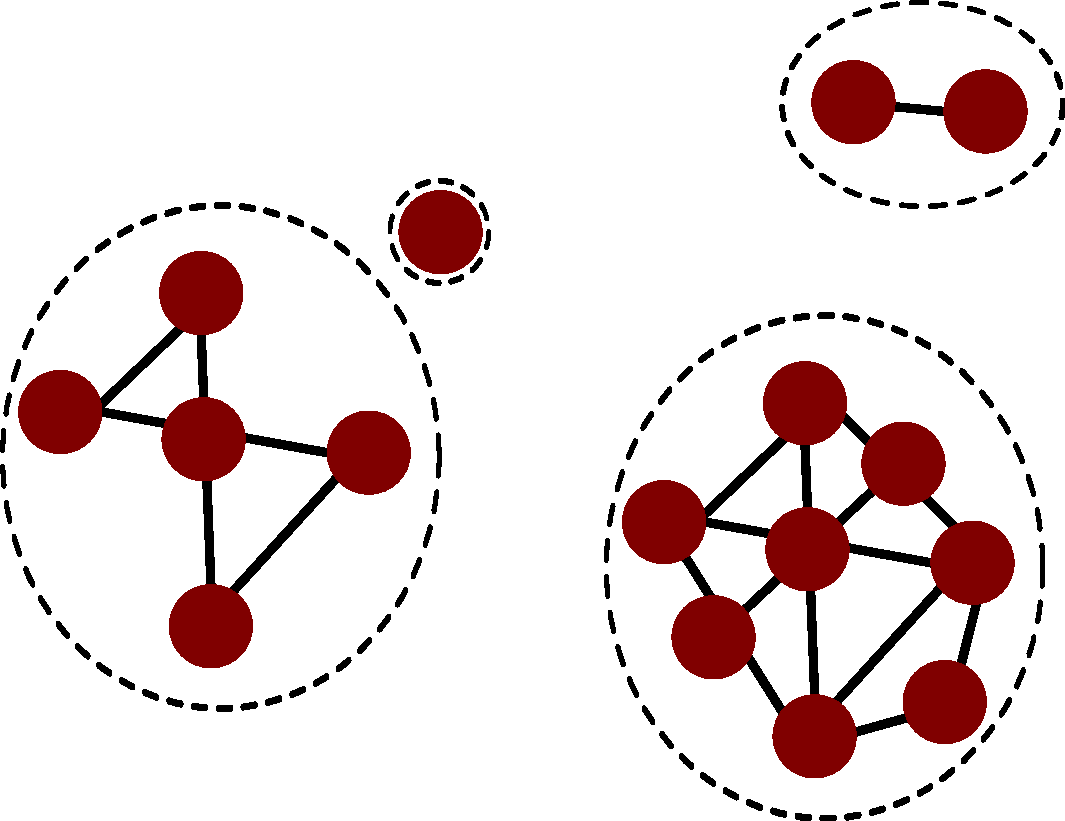
\includegraphics[height=3cm]{./imgs/store-carry-fwd-0.pdf}
      \caption{Store-carry-and-forward \cite{ieee12khabbaz}}
    \end{figure}
  \end{frame}
  \begin{frame}
    \frametitle{Bonus}
    \begin{figure}[p]
      \centering
      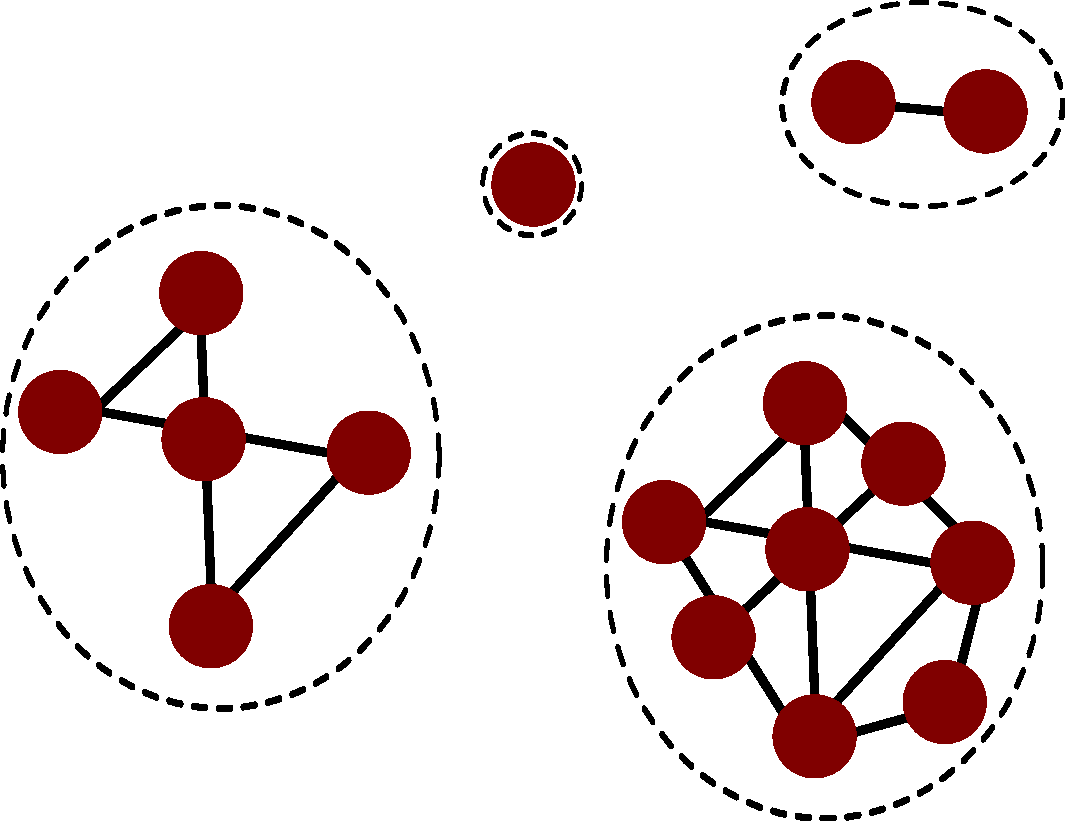
\includegraphics[height=3cm]{./imgs/store-carry-fwd-1.pdf}
      \caption{Store-carry-and-forward \cite{ieee12khabbaz}}
    \end{figure}
  \end{frame}
  \begin{frame}
    \frametitle{Bonus}
    \begin{figure}[p]
      \centering
      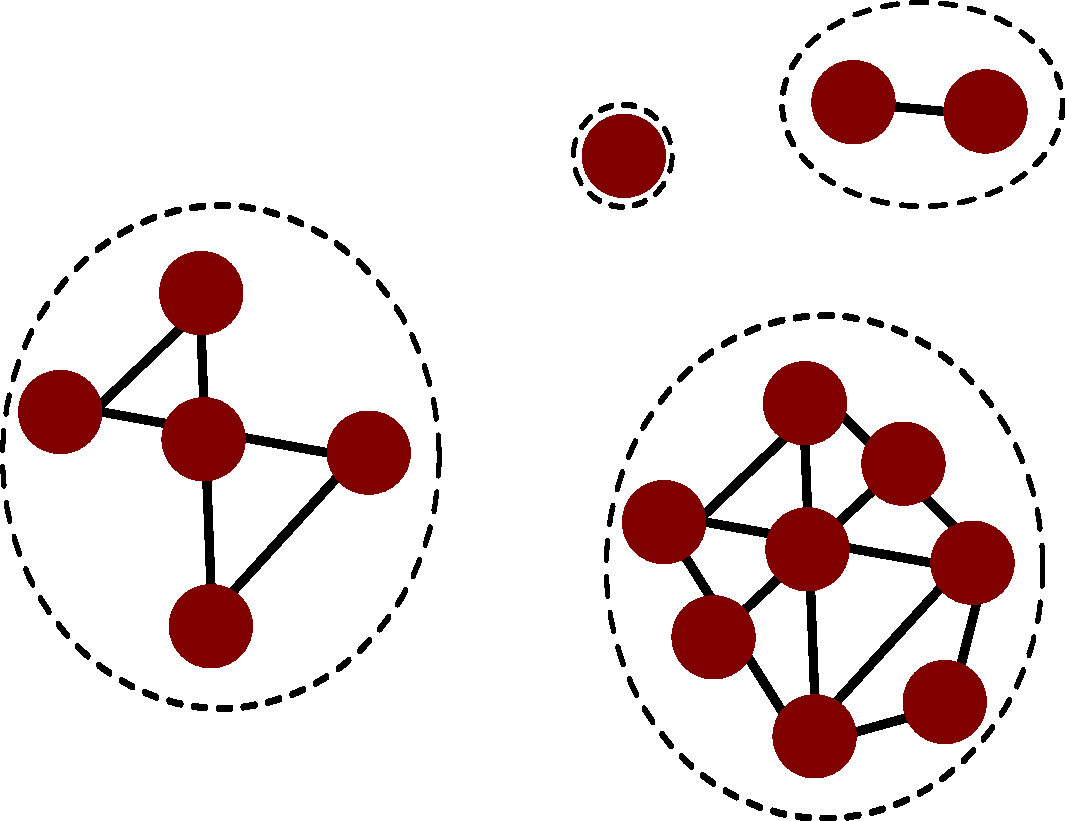
\includegraphics[height=3cm]{./imgs/store-carry-fwd-2.pdf}
      \caption{Store-carry-and-forward \cite{ieee12khabbaz}}
    \end{figure}
  \end{frame}
  \begin{frame}
    \frametitle{Bonus}
    \begin{figure}[p]
      \centering
      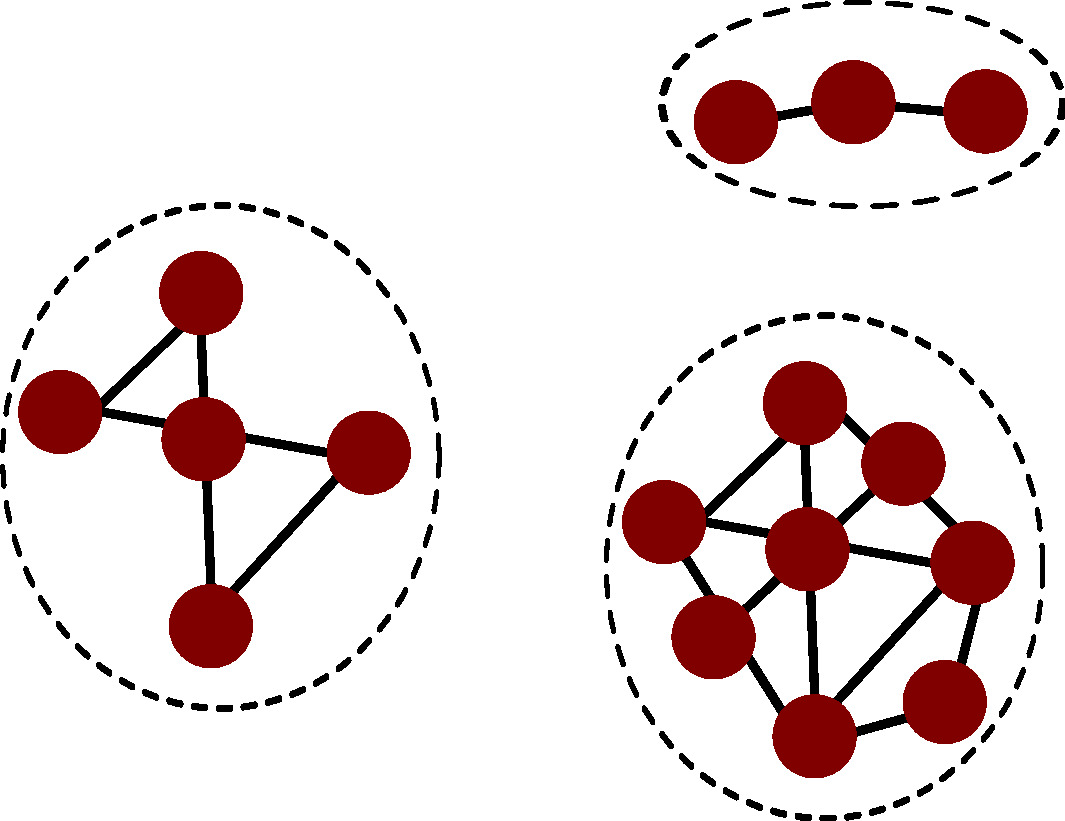
\includegraphics[height=3cm]{./imgs/store-carry-fwd-3.pdf}
      \caption{Store-carry-and-forward \cite{ieee12khabbaz}}
    \end{figure}
  \end{frame}


\subsection{HTTP request/response example}
\begin{frame}
    \frametitle{HTTP request/response example}
      Enter \color{blue}\href{http://getbootstrap.com}{getbootstrap.com} \color{black} in your browser\pause
      \begin{figure}
    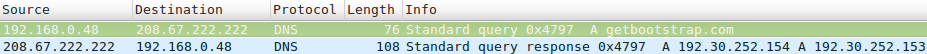
\includegraphics[width=11.5cm]{./imgs/dns-req.png}
  \caption{DNS request/response}
      \end{figure}
      \pause
      \begin{figure}
    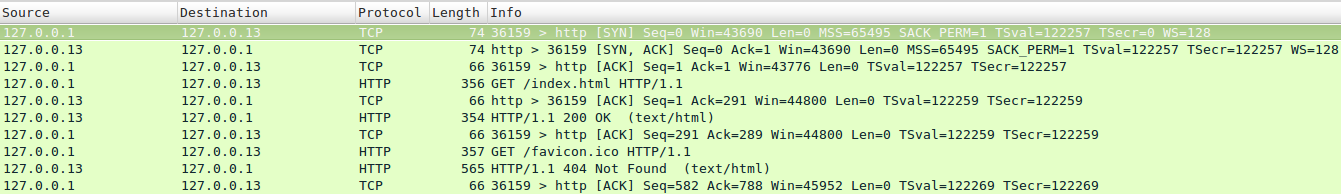
\includegraphics[trim = 0 0 100mm 0, clip, width=11.5cm]{./imgs/http-req.png}
  \caption{HTTP request/response}
      \end{figure}
  \end{frame}
    \begin{frame}
    \frametitle{How do messages reach their destination?}
      \begin{figure}
    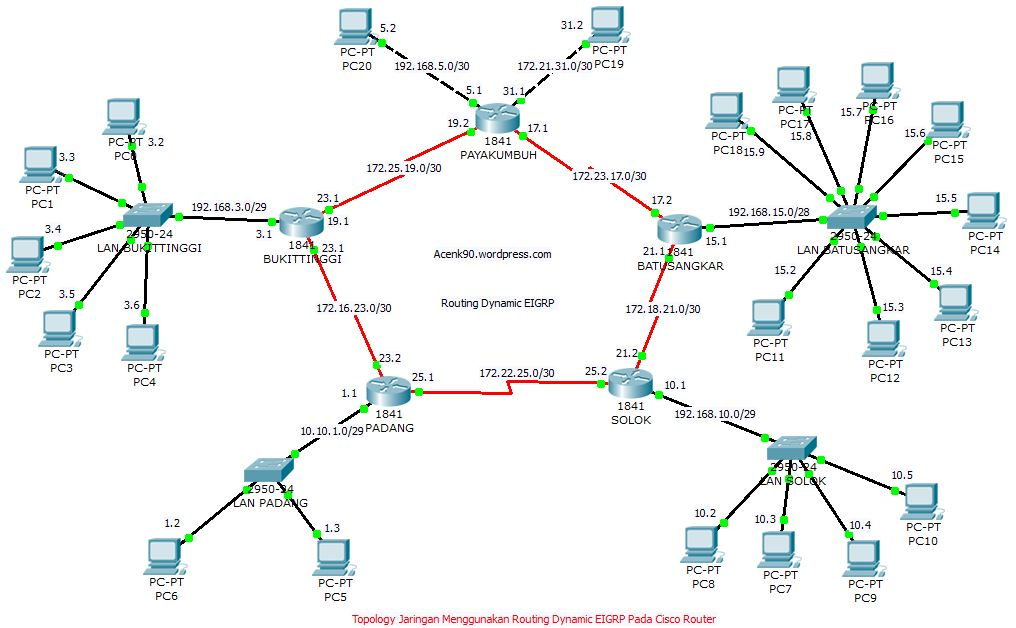
\includegraphics[width=9.5cm]{./imgs/routing.jpg}
  \caption{\color{blue}\href{http://acenk90.files.wordpress.com}{acenk90.files.wordpress.com}}
  \label{fig:routing}
      \end{figure}
  \end{frame}
    \begin{frame}
    \frametitle{More like this...}
      \begin{figure}
    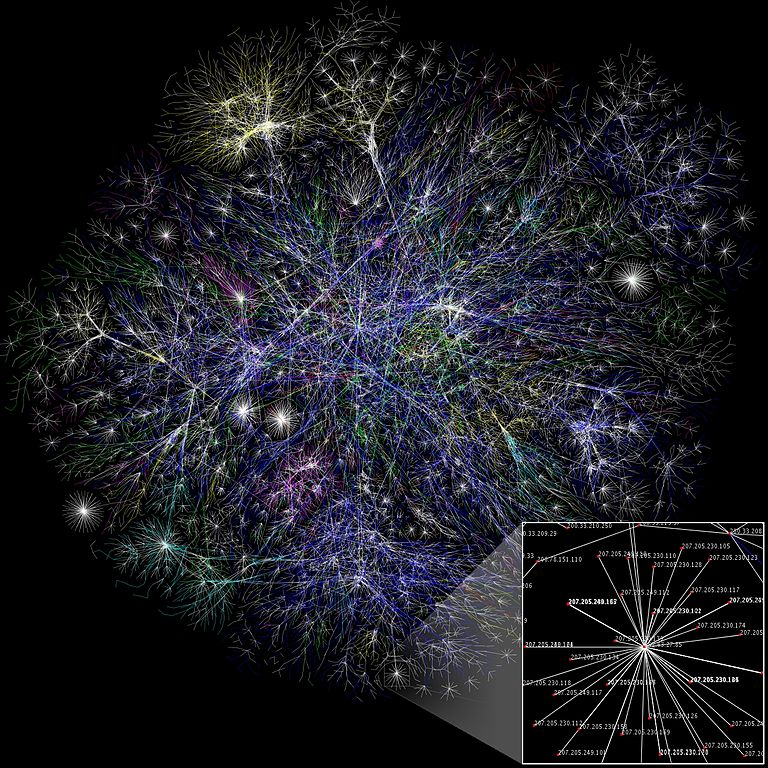
\includegraphics[height=6.5cm]{./imgs/map.jpg}
  \caption{\color{blue}\href{https://upload.wikimedia.org/wikipedia/commons/thumb/d/d2/Internet_map_1024.jpg/768px-Internet_map_1024.jpg}{wikimedia.org}}
  \label{fig:map}
      \end{figure}
  \end{frame}

\subsection{Models overview (OSI and TCP/IP)}
  \begin{frame}
    \frametitle{How does it work? From signal to application...}
    \begin{figure}[t]
      \centering
      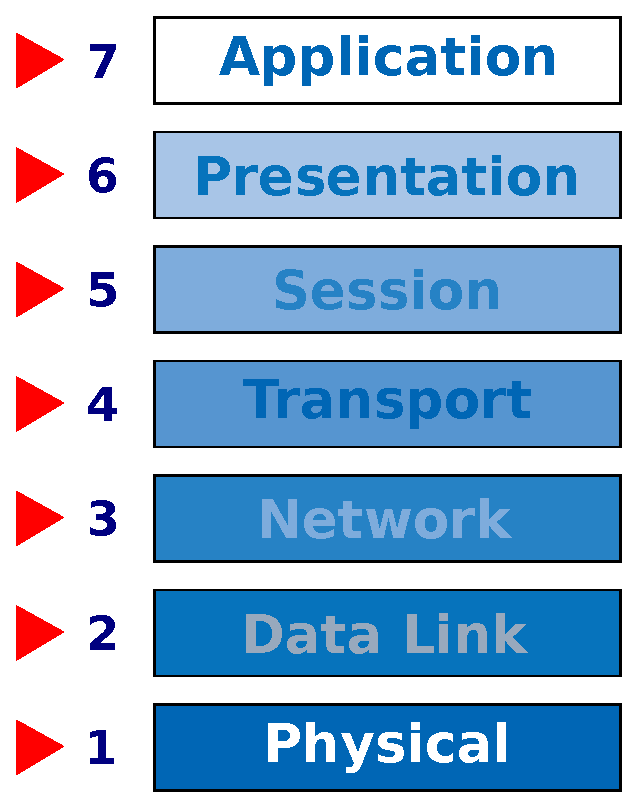
\includegraphics[height=6cm]{./imgs/osi_model.eps}
      \caption{OSI model}
      \label{fig:osi_mod}
    \end{figure}
  \end{frame}
  \begin{frame}
    \frametitle{N\textsuperscript{th} layer communicate with N\textsuperscript{th} layer..}
    \begin{figure}[t]
      \centering
      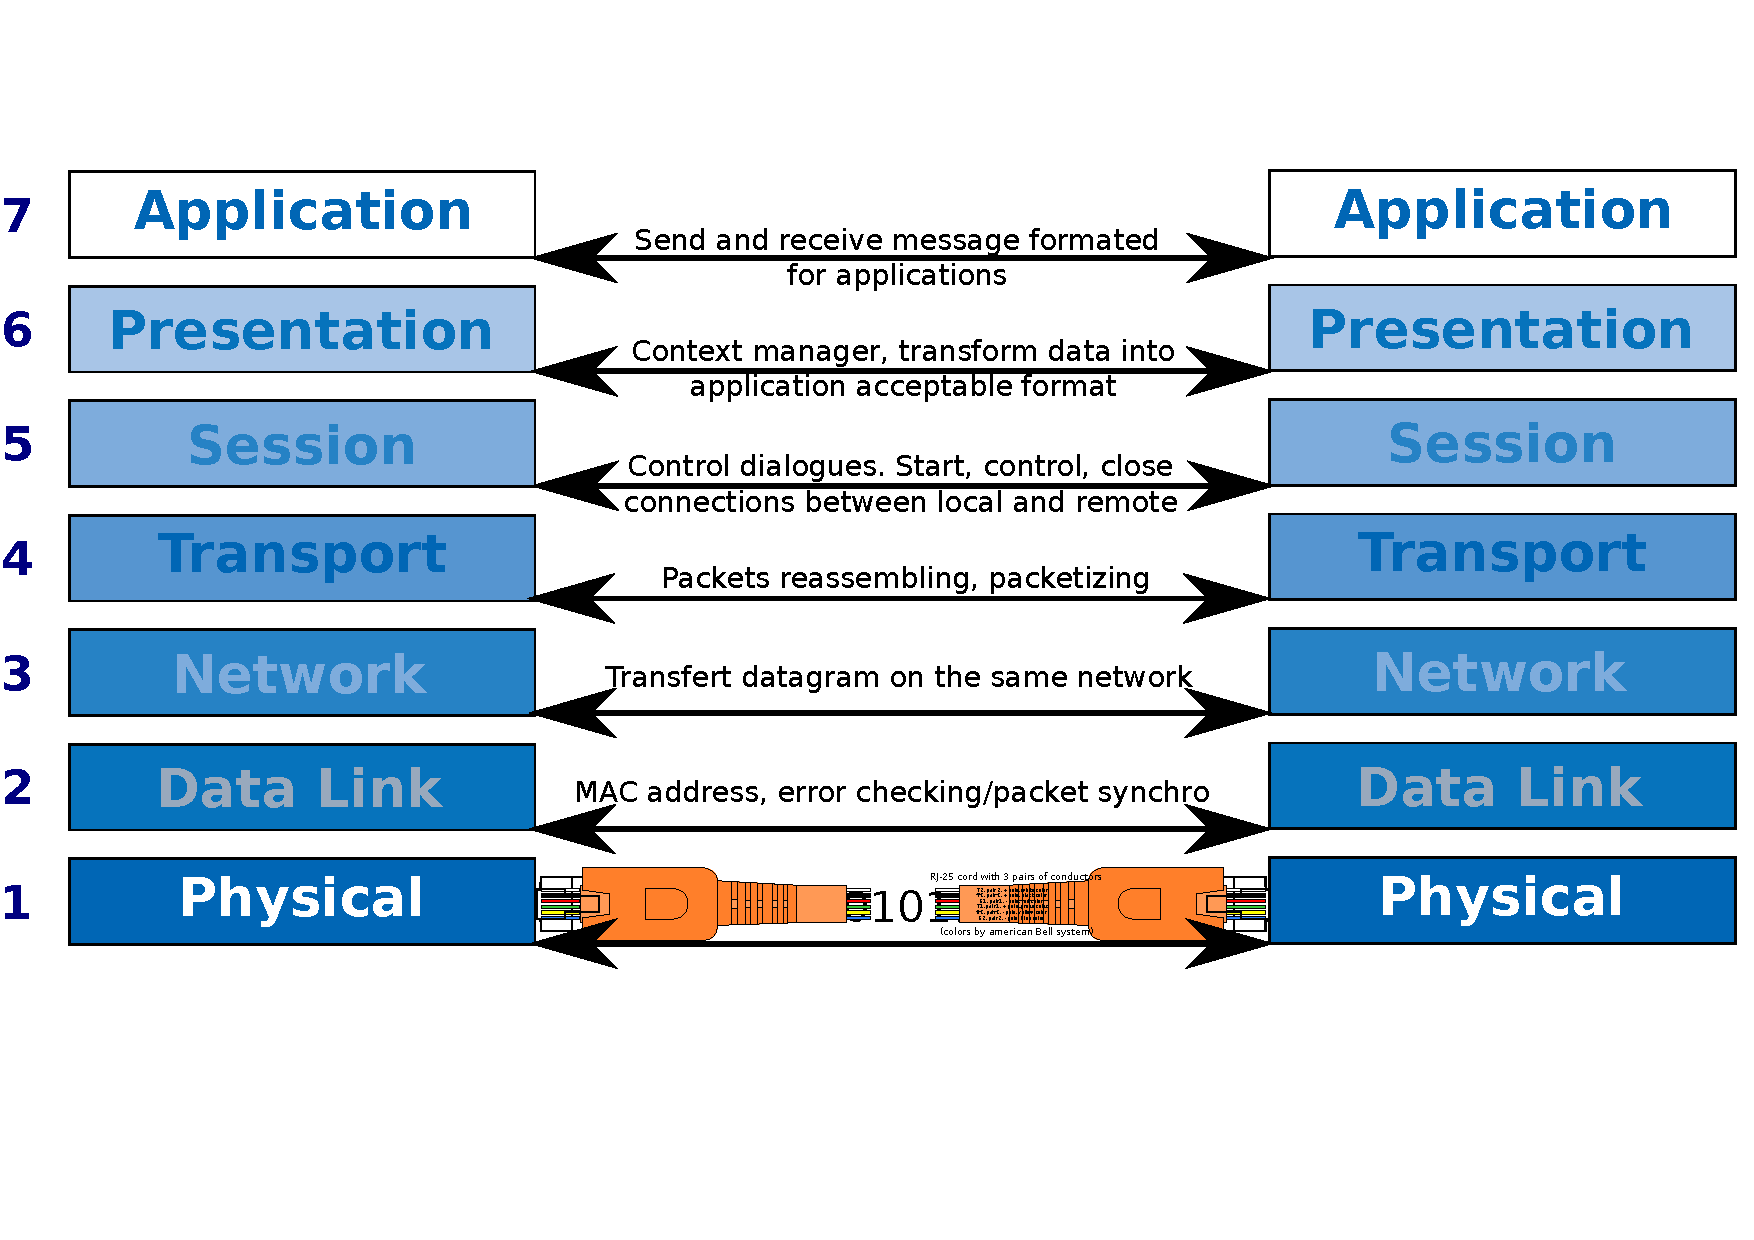
\includegraphics[height=7.5cm]{./imgs/layer2layer.pdf}
      \caption{layer to layer}
      \label{fig:layer2layer}
    \end{figure}
  \end{frame}
  \begin{frame}
    \frametitle{.. thanks to 3-\textsuperscript{th} layers}
    \begin{figure}[t]
      \centering
      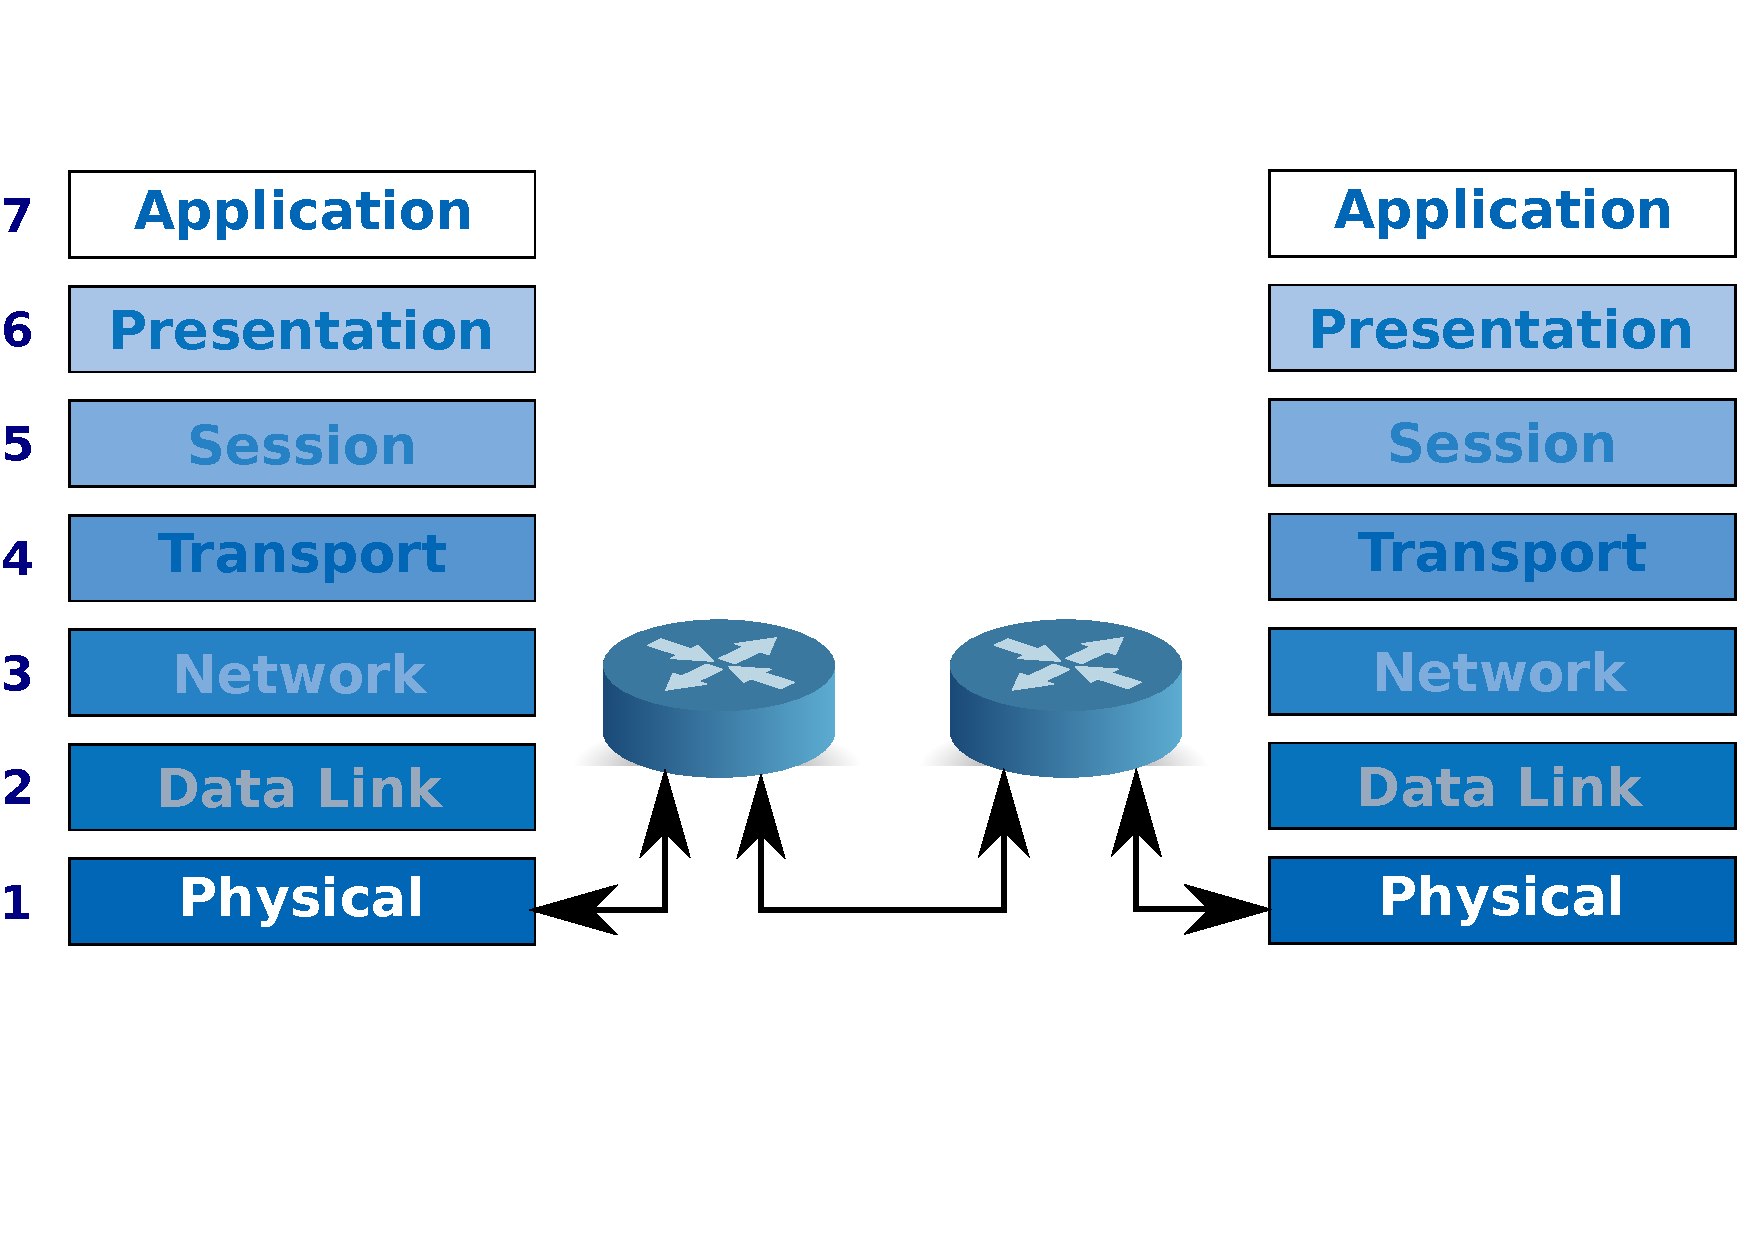
\includegraphics[height=7.5cm]{./imgs/layers_routers.pdf}
      \caption{layers and routing}
      \label{fig:layers_routing}
    \end{figure}
  \end{frame}
  \begin{frame}
    \frametitle{One single protocol, one single layer}
    \begin{figure}[t]
      \centering
      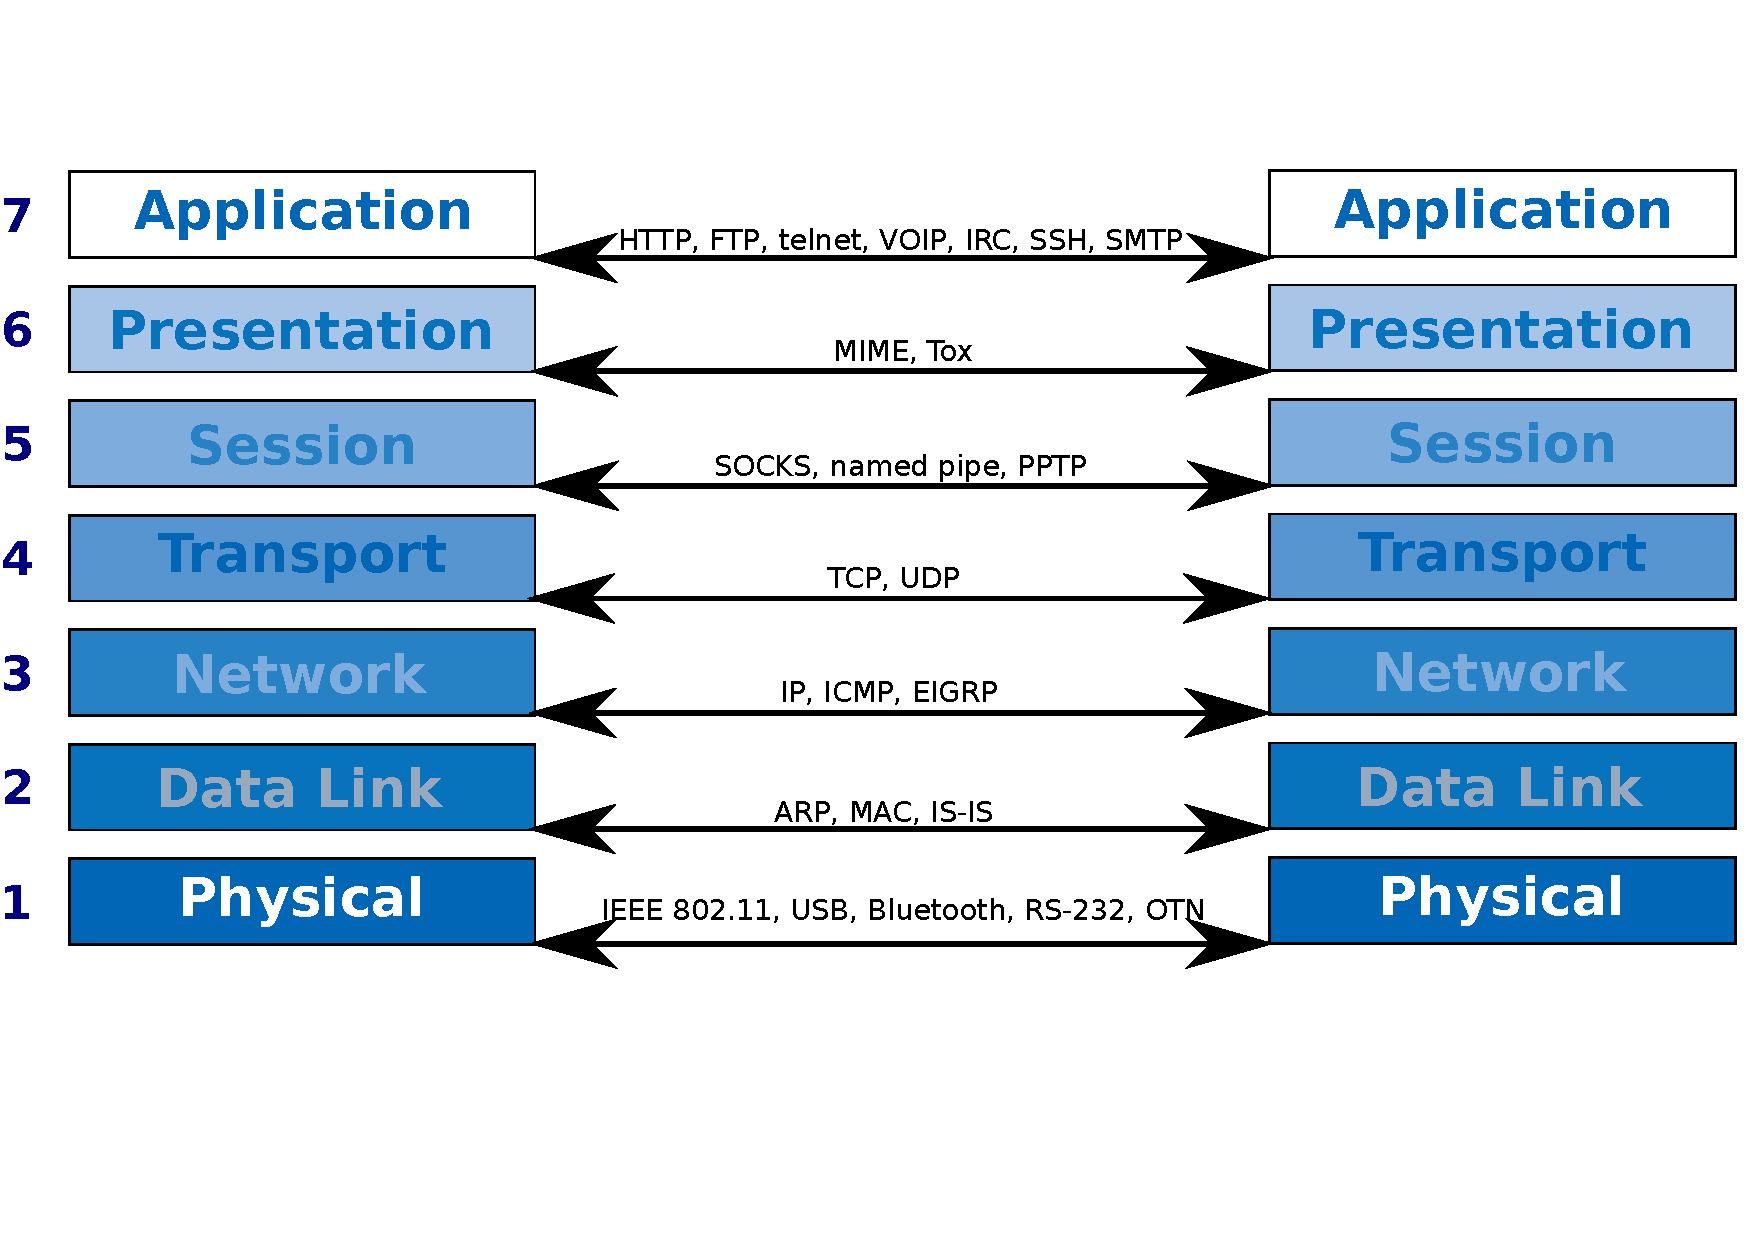
\includegraphics[height=7.5cm]{./imgs/layer2protocol.pdf}
      \caption{protocols and layers}
      \label{fig:layers2proto}
    \end{figure}
  \end{frame}
  \begin{frame}
    \frametitle{Encapsulation}
    \begin{figure}[t]
      \centering
      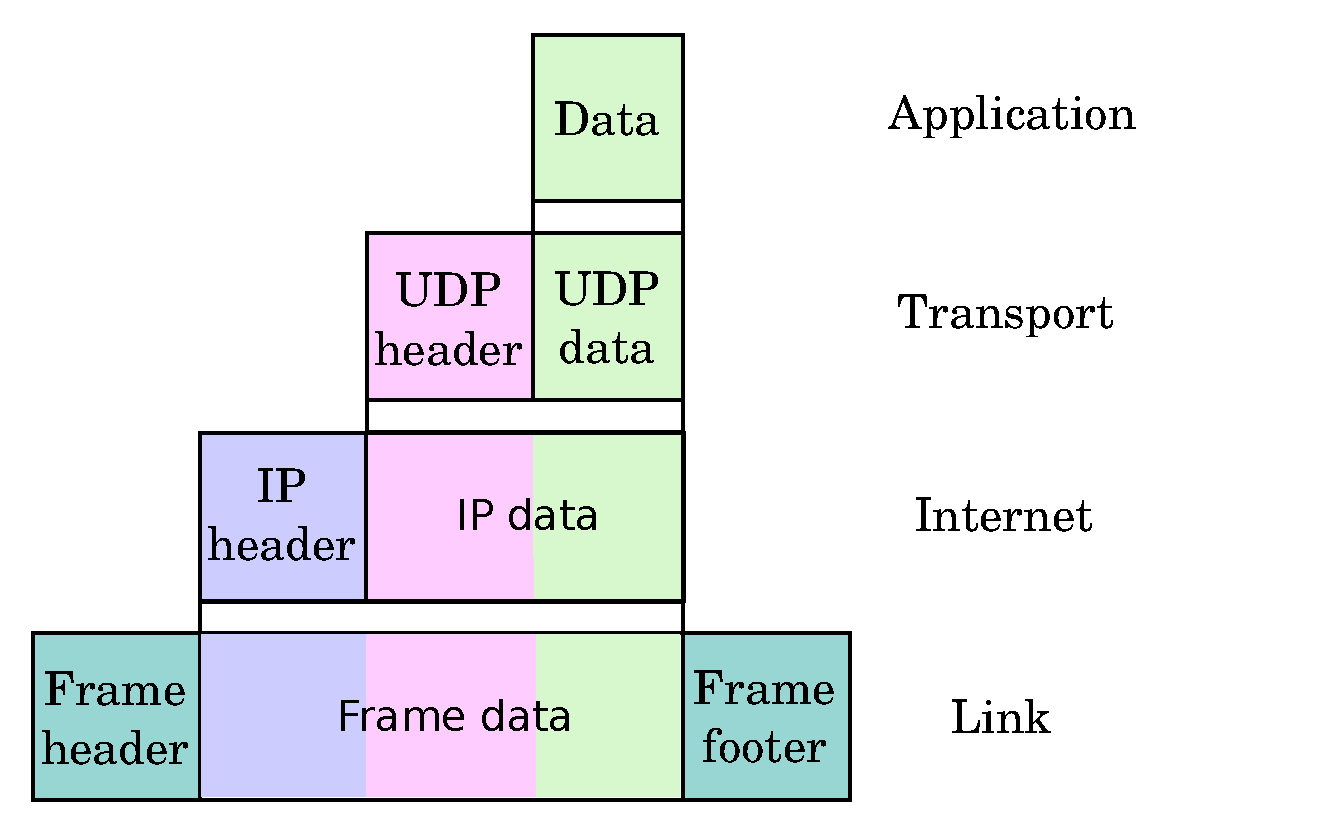
\includegraphics[height=7.5cm]{./imgs/encapsulation.pdf}
      \caption{Encapsulation}
      \label{fig:encapsulation}
    \end{figure}
  \end{frame}

\section{Lower layers}
  \begin{frame}
    \frametitle{From analog/logical signals up to messages}
  \end{frame}
\subsection{Physical}
  \begin{frame}
    \frametitle{}
  \end{frame}
\subsection{Data Link}
  \begin{frame}
    \frametitle{Course details}
  \end{frame}
\subsection{Network}
  \begin{frame}
    \frametitle{Course details}
  \end{frame}
\subsection{Transport}
  \begin{frame}
    \frametitle{Course details}
  \end{frame}

\subsection{Session}
  \begin{frame}
    \frametitle{Course details}
  \end{frame}
\subsection{Presentation}
  \begin{frame}
    \frametitle{Course details}
  \end{frame}
\subsection{Application}
  \begin{frame}
    \frametitle{Course details}
  \end{frame}

\section*{Conclusion}
  \begin{frame}
    \frametitle{References}
    \bibliography{ref.bib}
  \end{frame}
\end{document}
